% !TEX program = xelatex
%% Requires compilation with XeLaTeX or LuaLaTeX
\documentclass[10pt,xcolor={table,dvipsnames},t]{beamer}
\usepackage{biblatex}
\usepackage{caption}
\setbeamertemplate{caption}[numbered]
\addbibresource{reference.bib}
\usepackage{hyperref}
\hypersetup{
pdfpagemode=FullScreen,  
colorlinks=true,linkcolor=blue}
\usepackage{enumerate}
\usepackage{algorithm}
\usepackage{algpseudocode}
\usepackage{listings}
\usepackage{xcolor}
\usepackage{graphicx}

\definecolor{codegreen}{rgb}{0,0.6,0}
\definecolor{codegray}{rgb}{0.5,0.5,0.5}
\definecolor{codepurple}{rgb}{0.58,0,0.82}
\definecolor{backcolour}{rgb}{0.95,0.95,0.92}

\lstdefinestyle{mystyle}{
    backgroundcolor=\color{backcolour},   
    commentstyle=\color{codegreen},
    keywordstyle=\color{magenta},
    numberstyle=\tiny\color{codegray},
    stringstyle=\color{codepurple},
    basicstyle=\ttfamily\footnotesize,
    breakatwhitespace=false,         
    breaklines=true,                 
    captionpos=b,                    
    keepspaces=true,                 
    numbers=left,                    
    numbersep=5pt,                  
    showspaces=false,                
    showstringspaces=false,
    showtabs=false,                  
    tabsize=2
}

\lstset{style=mystyle}

% Flow chart config
\usepackage{tikz}
\usetikzlibrary{calc,trees,positioning,arrows,fit,shapes,calc,tikzmark,matrix}
\usepackage{eso-pic}
\usetikzlibrary{shapes.geometric, arrows}
\tikzstyle{startstop} = [rectangle, rounded corners, minimum width=3cm, minimum height=1cm,text centered, draw=black, fill=red!30]
\tikzstyle{io} = [trapezium, trapezium left angle=70, trapezium right angle=110, minimum width=3cm, minimum height=1cm, text centered, draw=black, fill=blue!30]
\tikzstyle{process} = [rectangle, minimum width=3cm, minimum height=1cm, text centered, draw=black, fill=orange!30]
\tikzstyle{decision} = [diamond, minimum width=3cm, minimum height=1cm, text centered, draw=black, fill=green!30]
\tikzstyle{arrow} = [thick,->,>=stealth]

\usetheme{UCBerkeley}

\title[Your Short Title]{STMC coding team Training}
\subtitle{Lesson 7: More On Problem Solving}
\author{Tsai Yun Chen}
%\institute{}
\date{\today}

\begin{document}

\begin{frame}
  \titlepage
\end{frame}

% Uncomment these lines for an automatically generated outline.
%\begin{frame}{Outline}
%  \tableofcontents
%\end{frame}

\section{Class Goal}

\begin{frame}{Goal today}
Today we will continue to look into solving some real life problems using all the thing taught so far.
\begin{itemize}
  \item Maze Game
  \item Maze Game with Shortest Path
  \item Maze Game with Weighted Shortest Path
\end{itemize}
\end{frame}


\section{Recap}
\begin{frame}[fragile]{A brief recap}
  \begin{itemize}
    \item We solved two intersting problems last week
    \begin{itemize}
      \item the Hanoi Tower
      \item the (0-1) Knapsack Problem
    \end{itemize}
    \item We learnt some techniques in solving those problems
    \begin{itemize}
      \item Greedy Algorithm
      \item Dynamic Programming
    \end{itemize}
    \item Today we will see some more intersting application of these two techniques
  \end{itemize}
\end{frame}

\begin{frame}{The Maze Game}
  \begin{itemize}
    \item Consider you are in a large field of $m\times n$ grids
    \item you standing at the top-left corner
    \item the exit is at the bottom-right corner
    \item There are obstacles on some of the grids
    \item you can only move right or down, one grid at a time
    \item Problem: Can you find the way out?
  \end{itemize}
\end{frame}

\begin{frame}{Task Description}
\begin{itemize}
\item We would like to program an algorithm that tell you either the way out or there is no way out
\item Input: The maze, expressed as a list of list
\begin{itemize}
  \item your position is marked as u, initially at the top-left corner
  \item obstacles are marked as o, can 0, 1, or more than 1
  \item exit is marked a e, initially at the bottom-right corner
\end{itemize}
\item Output: The list of grids to be visited, or ``NO WAY OUT'' if there is no way to reach the end
\end{itemize}
\end{frame}

\begin{frame}[fragile]{First Trial}
\begin{itemize}
\item Sometimes simple is the best
\item Since we have at most two choices at each grid, we can try all of them
\item Let's try to code it!
\begin{lstlisting}[language=python]
  def MazeSolver(maze):
    #the maze is expressed as a list of list
    ###your code start below###

  #Then we ask the user to provide the number of pile to be solved, and call the function we just implemented.
  SampleMaze = [['u',' ',' '],[' ','o',' '],[' ',' ','e']]
  MazeSolver(SampleMaze)
\end{lstlisting}
\item Problem: How long does it takes to try all? Let's say for a $3\times 3$ field with obstacle in the middle.
\end{itemize}
\end{frame}

\begin{frame}{Simple Improvement}
  \begin{itemize}
    \item We are looking into the same grids more than once!
    \item How can we avoid that?
    \item Observation: If we can reach exit from a certain grid, then we must already returned the solution!
    \item So all visited grids have no solution, therefore no need to check again
    \item Idea: Create a boolean table, same as the size of the maze, to mark whether the grid has been checked or not
    \item Problem: How to implement it? Let's try!
  \end{itemize}
\end{frame}

\begin{frame}[fragile]{Shortest Path Problem}
  \begin{itemize}
    \item What we have just done is called the Depth-First Search (DFS), it's also kind of Greedy Algorithm
    \item Just as last time, it's simple to think, and simple to implement
    \item But... It's not optimal, also become slow when it becomes more complicated
    \item Let's assume the exit no longer stay at the bottom right corner
    \item Also we are now free to move in all four direction
    \item Consider now we are not only to find the way out, we want to find the shortest way possible
    \item What can we do?
  \end{itemize}
\end{frame}

\begin{frame}[fragile]{What if there is more than one people?}
  \begin{itemize}
    \item Let's assume, instead of only you, your friends are in the maze as well
    \item Another assumption, if one of you get out, all of you are free
    \item Can we do better?
    \item We can try multiple path at the same time!
    \item Problem: How can we simulate that in our computer?
    \item We can't really compute various things at the same time (actually we can, but that's hard)
    \item But ... we can simulate that using looping
  \end{itemize}
\end{frame}

\begin{frame}{Looping with Visit Queue}
  \begin{itemize}
    \item To achive that, we maintain a list named VisitQueue
    \item Initially the VisitQueue contains only the initial position
    \item At each loop, it is simulating a group of people on a certain grid
    \item Then as we need to send people to other grid
    \item We add all possible direction of walking to the end of the VisitQueue
    \item As soon as the loop visited the target, we are done
  \end{itemize}
\end{frame}

\begin{frame}[fragile]{Implementation}
\begin{lstlisting}[language=python]
  def MazeSolver(maze):
    m = len(maze)
    n = len(maze[0])
    Visited = [[False * n]*m]
    VisitQueue = [(0,0)]
    for pos in VisitQueue:
      Visited[pos[0]][pos[1]] = True
      if maze[pos[0]][pos[1]] == 'e':
        return "Found the way out!"
      if pos[0]>0 and not Visited[pos[0]-1][pos[1]] and maze[pos[0]-1][pos[1]] != 'o':
        VisitQueue.append((pos[0]-1,pos[1]))
      if pos[1]>0 and not Visited[pos[0]][pos[1]-1] and maze[pos[0]][pos[1]-1] != 'o':
        VisitQueue.append((pos[0],pos[1]-1))
      if pos[0]<m-1 and not Visited[pos[0]+1][pos[1]] and maze[pos[0]+1][pos[1]] != 'o':
        VisitQueue.append((pos[0]+1,pos[1]))
      if pos[1]<n-1 and not Visited[pos[0]][pos[1]+1] and maze[pos[0]][pos[1]+1] != 'o':
        VisitQueue.append((pos[0],pos[1]+1))
    return "No Way Out!"
\end{lstlisting}
\end{frame}

% \begin{frame}[fragile]{Example}
%   \begin{figure}
%     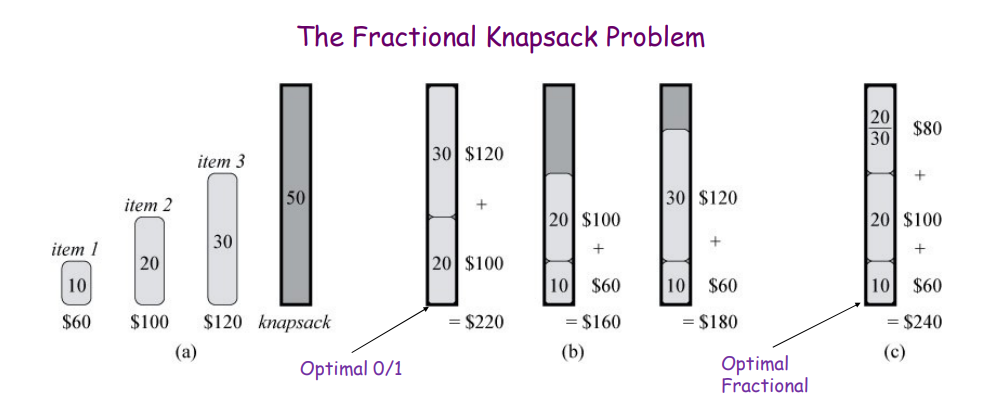
\includegraphics[width=0.8\textwidth]{img/knapsack.png}
%   \end{figure}
% \end{frame}

\begin{frame}{Challenge I}
  \begin{itemize}
    \item The code in checking whether we can append a certain position into the VisitQueue is quite annoying and redundant
    \item Can you write a simple function and replace those lines with the function?
    \item Design your own function, include naming and parameter needed
    \item try to make it as simple as possible
  \end{itemize}
  \end{frame}

\begin{frame}{Challenge II}
  \begin{itemize}
    \item Recall in the original version of the task, we need to obtain the path to the exit
    \item Here we only answer whether there is a way out
    \item Can you modify the code so that it also return the code whenever the exit is reachable?
    \item Idea: Instead of a single position, maintain a list of position in the queue
  \end{itemize}
  \end{frame}

\begin{frame}[fragile]{Challenge III}
  \begin{itemize}
    \item Now consider the exit is locked
    \item You need to find the key before moving to the exit, which is marked as 'k' in the field
    \item How can we find the new shortest path for this?
  \end{itemize}
\end{frame}

\begin{frame}[fragile]{Challenge IV}
  \begin{itemize}
    \item Continue with the previous setting, the exit is locked
    \item Now the floor of each grid will disappear after you walked over it, there is lava below it
    \item This means you cannot walk through the same grid twice
    \item Now how do you find the new shortest path?
  \end{itemize}
\end{frame}

\end{document}
